\documentclass[a4paper]{article}
\usepackage[utf8]{inputenc}
\usepackage[toc,page]{appendix}
\usepackage{graphicx}
\usepackage{epsfig}
\usepackage{color}
\usepackage{array}
\usepackage{lscape}
\usepackage{calc}
\usepackage{hhline}
\usepackage{pslatex}
\usepackage{verbatim}
\usepackage{proof}
\usepackage[top=3cm, bottom=3cm, left=3.5cm, right=3.5cm]{geometry}
\usepackage{amsmath}
\usepackage{amssymb}
\usepackage{listings}
\hyphenation{where}

% Messy redefinition of caption font -
\newcommand{\captionfonts}{\small}
\makeatletter  % Allow the use of @ in command names
\long\def\@makecaption#1#2{%
  \vskip\abovecaptionskip
  \sbox\@tempboxa{{\captionfonts #1: #2}}%
  \ifdim \wd\@tempboxa >\hsize
    {\captionfonts #1: #2\par}
  \else
    \hbox to\hsize{\hfil\box\@tempboxa\hfil}%
  \fi
  \vskip\belowcaptionskip}
\makeatother   % Cancel the effect of \makeatletter

\newcommand{\buzz}[1]{{\sl #1}}
\newcommand{\code}[1]{{\tt #1}}

\newcommand{\lsb}{[\![}
\newcommand{\rsb}{]\!]}
\newcommand{\pipe}{\ | \ }

\newcommand{\s}[1]{\mathtt{#1}}
\newcommand{\sn}{\overline{n}}
\newcommand{\sx}{\s{n}}
\newcommand{\sLp}{\s{(}}
\newcommand{\sRp}{\s{)}}
\newcommand{\sLb}{\s{\{}}
\newcommand{\sRb}{\s{\}}}
\newcommand{\sbool}{\s{bool\ }}
\newcommand{\sint}{\s{int\ }}
\newcommand{\sseta}{\s{set\ }}
\newcommand{\sLa}{\s{\langle}}
\newcommand{\sRa}{\s{\rangle}}
\newcommand{\swhile}{\s{\ while\ }}
\newcommand{\sif}{\s{if\ }}
\newcommand{\sthen}{\s{\ then\ }}
\newcommand{\selse}{\s{\ else\ }}
\newcommand{\sifthenelse}[3]{\sif #1 \sthen #2 \selse #3}
\newcommand{\spick}[3]{\s{pick}\ #1\ \s{some}\ #2\ \s{none}\ #3}
\newcommand{\srepeat}{\s{\ repeat\ }}
\newcommand{\suntil}{\s{\ until\ }}
\newcommand{\scase}{\s{\ case\ }}
\newcommand{\sof}{\s{\ of\ }}
\newcommand{\slet}{\s{\ let\ }}
\newcommand{\sletin}[2]{\s{let\ } #1 \s{\ in\ } #2}
\newcommand{\srec}{\s{rec\ }}
\newcommand{\sskip}{\s{skip}}
\newcommand{\strue}{\s{true}}
\newcommand{\sfalse}{\s{false}}
\newcommand{\seq}{\s{=\ }}
\newcommand{\sfn}{\s{fn}\ }
\newcommand{\fst}[1]{\ \s{fst}(#1)}
\newcommand{\snd}[1]{\ \s{snd}(#1)}
\newcommand{\sset}[1]{\sLb #1 \sRb}
\newcommand{\ssetc}[1]{\sset{#1}_{\!\!\!\surd}}

\newcommand{\biim}{\Leftrightarrow}
\newcommand{\im}{\Rightarrow}
\newcommand{\bim}{\Leftarrow}
\newcommand{\imback}{\Leftarrow}
\newcommand{\step}{\to}
\newcommand{\stepsub}{\step^{sub}}
\newcommand{\patbind}{\Rightarrow^{pat}}
\newcommand{\rstep}{\gets}
\newcommand{\steps}{\step^{*}}
\newcommand{\bstep}{\step_\beta}
\newcommand{\bsteps}{\steps_\beta}
\newcommand{\rbstep}{\ _\beta\!\gets}
\newcommand{\beq}{\leftrightarrow_\beta}
\newcommand{\bneq}{\nleftrightarrow_\beta}
\newcommand{\dotset}[2]{\{#1,\ldots,#2\}}
\newcommand{\angled}[1]{\langle #1\rangle}

\newcommand{\te}[1]{[#1]\vdash}
\newcommand{\tge}[1]{\Gamma[#1]\vdash}
\newcommand{\T}{\mathcal{T}}
\newcommand{\E}{\mathcal{E}}
\renewcommand{\S}{\mathcal{S}}
\newcommand{\sbig}[3]{\sLa #1 , #2 \sRa\downarrow #3}
\newcommand{\ssmall}[3]{#1 \vdash #2 \step #3}
\newcommand{\ssmalls}[3]{#1 \vdash #2 \steps #3}
\newcommand{\noteover}[2]{\begin{array}{cc}{_{#2}}\\#1\end{array}}
\newcommand{\stackover}[2]{\stackrel{{#2}}{#1}}
\renewcommand{\rule}[3][]{\ \mbox{\textsc{#1 }}\dfrac{#2}{#3}\ }
\newcommand{\smbox}[1]{
  $\begin{array}{|c|}
    \hline
    #1 \\
    \hline
  \end{array}$
}

\newcommand{\estep}{\stackrel{\epsilon}{\to}}

\newcommand{\sugar}[2]{\langle#2\rangle_{\mathcal{#1}}}
\newcommand{\sug}[1]{\sugar{E}{#1}}

\newtheorem{lemma}{Lemma}[section]

\title{FQL - A functional query language}
\date{August 2009}

\author{Joakim Ahnfelt-Rønne \and Mikkel Jønsson Thomsen \and Michael Werk}

\begin{document}
\parindent=0pt
\parskip=8pt plus 2pt minus 4pt
\maketitle

\begin{abstract}\noindent
A task has been assigned by an ERP systems vendor to formulate a functional language with embedded query constructs intended to extract data in the existing ERP system. The language is to be used as an abstraction between the ERP system and the relational database and must provide type safety in its core as well as in it's querie constructs by using a static type system. The core language is required to have tuples and sets as built-in data types, be parametrically polymorphic and include higher-order functions. In response to this request we here suggest the language FQL.
\end{abstract}


\section{Introduction}

FQL in it's core is simply types lambda calculus with a monomorph recursion constrict and support for polymorphic let bindings. The language hase integers and booleans as primitive types and pairs and sets as build-in structural types.


In this section we present the FQL, a functional query language for relational databases. We will first go through the syntax of the language, then we will design semantic rules and finally design a type system.

\section{Syntax}
\label{sec:syntax}

\subsection{Abstract syntex}
\label{abstractSyntax}

The syntax of FQL consists of \emph{terms}, \emph{patterns} and \emph{canonical forms of terms}. The terms will be defined by $t$:
\begin{eqnarray*}
t & ::= & \sn \pipe \strue \pipe \sfalse \pipe x \pipe t_1 + t_2 \pipe t_1
= t_2 \pipe \sifthenelse{t_1}{t_2}{t_3} \\
& & \pipe (t_1,
t_2) \pipe \lambda p.t \pipe t_1 t_2 \pipe \sletin{x \seq t_1}{t_2}
\pipe \srec x.t \pipe \sset{t^{,*}} \pipe t_1 \cup t_2
\end{eqnarray*}
Where the patterns $p$ are defined by
\begin{eqnarray*}
p & ::= & \sn \pipe \strue \pipe \sfalse \pipe x \pipe (t_1, t_2) \pipe
\sset{} \pipe \sset{p} \pipe p \cup p
\end{eqnarray*}
As discussed in section \ref{sec:semantics} we need a subset of terms that are canonical. These are defined by $c$
\begin{eqnarray*}
c & ::= & \sn \pipe \strue \pipe \sfalse \pipe (c_1, c_2) \pipe \lambda
p.t \pipe \ssetc{c_1,\ldots,c_n}
\end{eqnarray*}

\subsection{Concrete syntax}
\label{sec:concreteSyntax}

The concrete syntax for set comprehension is sketched here as $s$:

\begin{eqnarray*}
s & ::= & \{ t : f \pipe c\} \pipe \{ t : f \}\\
f & ::= & p \s{\ in\ } t, f \pipe p \s{\ in\ } t\\
c & ::= & t, c \pipe t \\
\end{eqnarray*}

Note that p is a pattern and t is a term. The rules for translating
the concrete syntax to abstract syntax is sketched here as
$\sug{t}$:

\begin{eqnarray*}
\sug{\{t:f\}} & \Longrightarrow & \sug{\{t:f\ |\ \s{true}\}} \\
\sug{\{t:f\ |\ c\}} & \Longrightarrow &
\s{map\ }
(\lambda \sugar{CP}{f}. [\![ t ]\!])\
(\s{filter\ } (\lambda \sugar{CP}{f}. \sugar{MC}{c})\
\sugar{CV}{f})
\end{eqnarray*}
\begin{eqnarray*}
\sugar{CV}{p\s{\ in\ } t, f} & \Longrightarrow & \sug{t} \times \sugar{CV}{f} \\
\sugar{CV}{p\s{\ in\ } t} & \Longrightarrow & \sug{t}
\end{eqnarray*}
\begin{eqnarray*}
\sugar{CP}{p\s{\ in\ } t, f} & \Longrightarrow & (\sugar{P}{p}, \sugar{CP}{f}) \\
\sugar{CP}{p\s{\ in\ } t} & \Longrightarrow & p
\end{eqnarray*}
\begin{eqnarray*}
\sugar{MC}{t, c} & \Longrightarrow & \sug{t} \s{\ and\ } \sugar{MC}{c} \\
\sugar{MC}{t} & \Longrightarrow & \sug{t}
\end{eqnarray*}

In summary, we take the cross product of the input sets, pass it
through the well known filter function to apply the predicate,
and map it with the output function. We generate one big pattern
based on the patterns to the left of the input sets and use it as
the pattern for the predicate and output functions, thus binding
the values to the names as intended. An example of the concrete
syntax is
\begin{verbatim}
{(name, amount) : (name, accountnr) in owners,
                  (accountnr', amount) in accounts |
                  accountnr = accountnr'}
\end{verbatim}
which is translated to the abstract syntax
\begin{eqnarray*}
&&\s{map\ } (\lambda ((name, accountnr), (accountnr', amount)). (name, amount))\\
&&\quad(\s{filter\ } (\lambda ((name, accountnr), (accountnr', amount)). accountnr = accountnr')\\
&&\quad(owners \times accounts))
\end{eqnarray*}
This may be expressed more succinctly as
\begin{verbatim}
{(name, amount) : (name, accountnr) in owners,
                  (accountnr, amount) in accounts}
\end{verbatim}
Note that $accountnr$ is used twice here. The intention is that
both places in the pattern must match the same value
simultaneously, and the resulting abstract syntax is the same as
in the previous example. This can be implemented as syntactic sugar
by keeping track of which variables have been used before in the
set comprehension. In case a variable $x$ is encountered again in a
pattern, replace that occurrence with a fresh variable $x'$ and add
the constraint $x = x'$ to
the filter. For booleans, integers and other literals, they too can
be replaced by a constraint $c = x'$ where $c$ is the literal and
$x'$ is the fresh variable that replaced it in the pattern.



\section{Semantics}
\label{sec:semantics}

We present the semantics of FQL as a small step semantic by the judgment: \smbox{t \step t'}
\\
The binary relation $\oplus$ covers the stepping rules for $= ,+,\cup, \cap,\setminus,\in$, application and the pair construct.

Step rules.
\[\begin{array}{c}
\rule[S-Step1]{t_1 \step t_1'}{t_1 \oplus t_2 \step t_1' \oplus t_2}\quad
\rule[S-Step2]{t \step t'}{c \oplus t \step c \oplus t'}
\end{array}
\]

Addition of the numerals
\[
\rule[S-Plus]{}{\overline{n_1} \s{\ +\ } \overline{n_2} \step \overline{n_1 + n_2}}
\]

Primitive conditions
\[\begin{array}{c}
\rule[S-If1]{t_1 \step t_1'}{\sifthenelse{t_1}{t_2}{t_3} \step \sifthenelse{t_1'}{t_2}{t_3}}\\\\
\rule[S-IfL]{}{\sifthenelse{\strue}{t_2}{t_3} \step t_2}\quad
\rule[S-IfR]{}{\sifthenelse{\sfalse}{t_2}{t_3} \step t_3}
\end{array}\]

We define the let construct and general recursion as:
\[\begin{array}{c}
\rule[S-Let1]{t_1 \step t_1'}
  {\sletin{x=t_1}{t_2} \step \sletin{x=t_1'}{t_2}}\quad
\rule[S-Let]{}{\sletin{x=c}{t_2} \step [x \mapsto c ] t_2}\\\\
\rule[S-Rec]{}{\srec x.t \step [x \mapsto (\srec x.t)] t}
\end{array}\]


We use pattern matching to deconstruct the sets to resemble a query language.
In order to extract the bindings from the patterns we define the judgement \smbox{\angled{p,c} \stepsub S}
\[
\rule[SP-Var]{}{\angled{x,c} \stepsub [x\mapsto c]}\quad
\rule[SP-Pair]{\angled{p_1, c_1} \stepsub S_1 \quad \angled{p_2, c_2} \stepsub S_2}
{\angled{(p_1,p_2), (c_1, c_2)} \stepsub S_1S_2}
\]

Then we can define the rule for application
\[
\rule[S-App]{\angled{p, c} \stepsub S}{(\lambda p.t) c \step S(t)}
\]

Rules for equality of terms is only defined for terms of canonical forms. The interesting rules are the rules for the equality of sets. As sets are defined for all canonical terms $c$ we are able to have function terms $\lambda p.t$ in a set. If we define equality for sets, we either need to define equality for these terms or we need to exclude them from the sets. We then have two options:
\begin{enumerate}
\item terms $\lambda p.t$ are included in the sets and thus we need to define equality rules for these terms. It is however not possible to determine if two functions are equal, so either we would need some kind of identifier to determine equality or we need to define a static result of applying equality to functions i.e. true or false. The first solution will make similar functions appear unsimilar because they have different identifiers, thereby introducing the possibility of similar functions in a set and thereby conflicting with the mathematical definition of sets. The second solution have similar problems i.g. that if we define all functions to be equal, only one function can be present in a set and if we define all functions to be unequal, we again break the definition of the mathematical set.

\item We define sets to contain terms $c'$ where $c' ::= c \setminus \lambda p.t$ in which case we can define a \emph{canonical set} $\ssetc{c_1,\ldots,c_n}$ to only contain terms $c'$. By doing this we put a narrow restriction on the set type in exchange of preserving the properties of a mathematical set.
\end{enumerate}
By choosing option two we define equality as:
\[\begin{array}{c}
\rule[S-EqTT]{}{\strue = \strue \step \strue}
\quad
\rule[S-EqFF]{}{\sfalse = \sfalse \step \strue}
\quad\\\\
\rule[S-EqFT]{}{\sfalse = \strue \step \sfalse}
\quad
\rule[S-EqTF]{}{\strue = \sfalse \step \sfalse}
\quad\\\\
\rule[S-EqNT]{}{\overline{n} = \overline{n} \step \strue}
\quad
\rule[S-EqNF]{}{\overline{n_1} = \overline{n_2} \step \sfalse} (n_1 \neq n_2)
\quad\\\\
\rule[S-EqTupT]{c_1 = c_1' \step \strue \quad c_2 = c_2' \step \strue}
  {(c_1, c_2) = (c_1', c_2') \step \strue}
\quad\\\\
\rule[S-EqTupLF]{c_1 = c_1' \step \sfalse}
  {(c_1, c_2) = (c_1', c_2') \step \sfalse}
\quad
\rule[S-EqTupRF]{c_2 = c_2' \step \sfalse}
  {(c_1, c_2) = (c_1', c_2') \step \sfalse}
\quad\\\\
\rule[S-EqSetT]{\forall i \in \{1,\ldots,n\}. c_i \in  \ssetc{c'_1,\ldots,c'_n} \step \strue}
  {\ssetc{c_1,\ldots,c_n} = \ssetc{c'_1,\ldots,c'_n} \step \strue}
\quad\\\\
\rule[S-EqSetLF]{}{\ssetc{c_1,\ldots,c_n} = \ssetc{c'_1,\ldots,c'_m} \step \sfalse}(n \neq m)
\quad\\\\
\rule[S-EqSetF]{c_i \in \ssetc{c'_1,\ldots,c'_n} \step \sfalse}
  {\ssetc{c_1,\ldots,c_n} = \ssetc{c'_1,\ldots,c'_n} \step \sfalse}(i \in \{1,\ldots,n\})
\end{array}\]

In the following we present the semantic rules for set terms. The rule S-SetC is used to construct a canonical set from a semi-canonical set by deterministically reducing the set using rules S-SetR and S-SetS. We preserve the termination property by the rule S-SetC.

We define rules S-SetPickS and S-SetPickN to pick a member from a canonical set. As the sets are defined as mathematical sets, we do not provide any guarantees as to where the member is located in the set and again, the termination property is preserved by rule S-SetPickN. To provide a fail-safe semantic for the pick rules, we define the rule by using an \emph{option}-like construction to make it syntax driven.

\[\begin{array}{c}
\rule[S-Set1]{t_m \step t'_m}{\{c_1,\ldots,c_{m-1},t_m,\ldots,t_n\} \step \{c_1,\ldots,c_{m-1},t'_m,\ldots,t_n\} }
\quad\\\\
\rule[S-SetC]{\forall i \in \dotset{1}{n}.\forall j \in \dotset{1}{i-1,i+1,\ldots,n}. c_i = c_j \step \sfalse}
{\sset{c_1,\ldots,c_n} \step \ssetc{c_1,\ldots,c_n}}
\quad\\\\
\rule[S-SetR]{c_1 = c_i \step \strue}
{\sset{c_1,\ldots,c_n} \step \sset{c_2,\ldots,c_n}}(i \in \dotset{2}{n})
\quad\\\\
\rule[S-SetS]{\forall i \in \dotset{2}{n}. c_1 = c_i \step \sfalse
\quad c_j = c_k \step \strue}
{\sset{c_1,\ldots,c_n} \step \sset{c_2,\ldots,c_n,c_1}}(j,k \in \dotset{1}{n}, j\neq k)
\quad\\\\
\rule[S-SetIn1]{}{t_1\in t_2 \step t_1'\in t_2}
\quad
\rule[S-SetIn2]{}{c\in t \step c\in t'}
\quad\\\\
\rule[S-SetInT]{c=c_i \step \strue}{c\in \ssetc{c_1,\ldots,c_n} \step \strue}(i \in \dotset{1}{n})
\quad
\rule[S-SetInF]{\forall i\in\{1,\ldots,n\}. c=c_i \step \sfalse}{c_m \in \ssetc{c_1,\ldots,c_n} \step \sfalse}
\quad
\end{array}\]
\[\begin{array}{c}
\rule[S-SetPickN]{}{\spick{\ssetc{}}{(x_1,x_2) = t_1}{t_2} \step t_2}
\quad\\\\
\rule[S-SetPickS]{}{\spick{\ssetc{c_1,\ldots,c_n}}{(x_1,x_2) = t_1}{t_2} \step \sletin{x_1 = c_i}{(\sletin{x_2 = \sset{c_1,\ldots,c_n}\setminus\sset{c_i}}{t_1}})}
\quad\\\\
\rule[S-SetU]{}{\ssetc{c_1,\ldots,c_m} \cup \ssetc{c_{m+1},\ldots,c_n} \step
\{c_1,\ldots,c_m,c_{m+1},\ldots,c_n\}}
\quad\\\\
\rule[S-SetDT]{c_1 = c'_j \step \strue}
{\ssetc{c_1,\ldots,c_n} \setminus \ssetc{c'_1,\ldots,c'_j,\ldots,c'_m} \step
  \sset{c_2,\ldots,c_n} \setminus \sset{c'_1,\ldots,c'_{j-1},c'_{j+1},\ldots,c'_m}
}
\quad\\\\
\rule[S-SetDF]{\forall j \in \dotset{1}{m} c_1 = c'_j \step \sfalse}
{\ssetc{c_1,\ldots,c_n} \setminus \ssetc{c'_1,\ldots,c'_m} \step
  \sset{c_1} \cup (\sset{c_2,\ldots,c_n} \setminus \sset{c'_1,\ldots,c'_m})
}
\quad\\\\
\rule[S-SetDE]{}{\ssetc{} \setminus c \step \sset{}}
% This rule is not deterministec
%\rule{c_i = c'_j \step \strue}
%{\ssetc{c_1,\ldots,c_i,\ldots,c_m} \setminus \ssetc{c'_1,\ldots,c'_j,\ldots,c'_n} \step
%  \ssetc{c_1,\ldots,c_{i-1},c_{i+1},\ldots,c_m} \setminus \ssetc{c'_1,\ldots,c'_{j-1},c'_{j+1},\ldots,c'_n}
%}
% No longer required
%\quad\\\\
%\rule{\forall j \in \dotset{1}{n}. \forall i \in \dotset{1}{m}.   c_i = c'_j \step \sfalse}
%{\ssetc{c_1,\ldots,c_m} \setminus \ssetc{c'_1,\ldots,c'_n} \step
%  \ssetc{c_1,\ldots,c_m}
%}
\quad
\rule[S-SetI]{}{c_1 \cap c_2 \step (c_1 \cup c_2) \setminus ((c_1 \setminus c_2) \cup (c_2 \setminus c_1))}
\end{array}\]


With the \code{pick} construct in place, we can now define the aggregation function \code{reduce} as:
\[\begin{array}{l}
\srec \  reduce.\ \lambda f.\ \lambda z.\ \lambda s.\\
\quad \s{pick} \ s \\
\quad\quad \s{some} (e,r) = reduce \ f \ (f \  z \  e)\ r\\
\quad\quad \s{none} = z
\end{array}\]
We can also define fixed point queries by general recursion and set comprehension as:
\[\begin{array}{l}
\lambda f.\ \srec fix'.\ \lambda s.\\
\quad\quad\sletin{e = f\ s}{\sif e \setminus s = \{\} \sthen s \selse fix'\ (e \cup s)} \\
\end{array}\]
A concrete example of finding all nodes reachable from 1 would be:
\[\begin{array}{l}
\s{let\ } edges = \{(1, 2), (2, 3), (2, 4)\} \s{\ in}\\
\s{let\ } neighbors = \lambda v.\ \sLb y : (x,y) \s{\ in\ } edges \pipe x\in v \sRb\ \s{in} \\
\quad\quad fix\ neighbors\  \{1\}
\end{array}\]

The steps are sketched in figure \ref{figure:graph},
where the bold nodes are in the set.

\begin{figure}[h]
\centering
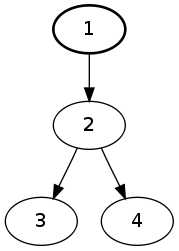
\includegraphics[width=0.15\textwidth]{grapha.png}
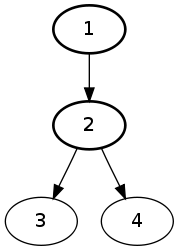
\includegraphics[width=0.15\textwidth]{graphb.png}
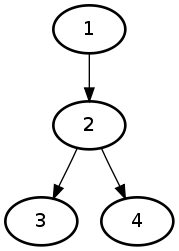
\includegraphics[width=0.15\textwidth]{graphc.png}
\caption{The three iterations in the reaching fixed point function.}
\label{figure:graph}
\end{figure}

\section{Type system}
\label{sec:typeSystem}

Types in FQL are defined by
\begin{eqnarray*}
\tau &::=& \sbool \pipe \sint \pipe \tau \to \tau \pipe \tau \times \tau \pipe \sseta \tau \pipe \alpha\\
\sigma &::=& \forall \alpha. \sigma \pipe \tau
\end{eqnarray*}
As discussed in section \ref{sec:semantics} we have to make sure
that every element in a set can be compared for equality. We define
a class of types that support this by the judgement
\smbox{\tau \in EQ}
\[\begin{array}{c}
\rule[EQ-Int]{}{\sint \in EQ}\quad
\rule[EQ-Bool]{}{\sbool \in EQ}\quad\\\\
\rule[EQ-Set]{}{\sseta \tau \in EQ}\quad
\rule[EQ-Pair]{\tau_1 \in EQ \quad \tau_2 \in EQ}{\tau_1 \times \tau_2 \in EQ}
\end{array}\]

We can then define the typing judgement
\smbox{\Gamma \vdash t : \tau}
and then formulate a syntax-oriented type system with constraint generation as side effects \cite{Heeren02generalizinghindley-milner, Henglein89polymorphictype}. We use side constraints to seperate the constraint generation from constraint solving because the constraint solution is independant of where the constrints come from \cite{henglein94fund-type-inf-sys}.

%The constraints are generated by rules T-App, T-Rec, T-Let, TP-Pair and T-Lam.

\[\begin{array}{c}
\rule[T-True]{}{\Gamma \vdash \strue : \alpha}(\alpha = \s{bool})\quad
\rule[T-False]{}{\Gamma \vdash \sfalse : \alpha}(\alpha = \s{bool})\quad
\\\\
\rule[T-Int]{}{\Gamma \vdash \sn : \alpha}(\alpha = \s{int})
\\\\
\rule[T-If]{\Gamma\vdash t_1 : \alpha_c \quad \Gamma\vdash t_2 : \alpha_t \quad \Gamma\vdash t_3 : \alpha_e}
{\Gamma\vdash \sif t_1 \sthen t_2 \selse t_3 : \alpha_i}
(\alpha_c = \s{bool} \wedge \alpha_i = \alpha_t \wedge \alpha_i = \alpha_e)
\\\\
\rule[T-Plus]{\Gamma\vdash t_1 : \alpha_1
\quad \Gamma\vdash t_2 : \alpha_2}
{\Gamma\vdash t_1 + t_2 : \alpha_+}
(\alpha_1 = \s{int} \wedge \alpha_2 = \s{int} \wedge \alpha_+ = \s{int})
\\\\
\rule[T-Eq]{\Gamma\vdash t_1 : \alpha_1
\quad \Gamma\vdash t_2 : \alpha_2}
{\Gamma\vdash t_1 = t_2 : \alpha_e}
(\alpha_e = \s{bool} \wedge \alpha_1 = \alpha_2 \wedge \alpha_1 \in EQ)
\\\\
\rule[T-Pair]{\Gamma\vdash t_1 : \alpha_1
\quad \Gamma \vdash t_2 : \alpha_2}
{\Gamma \vdash (t_1, t_2) : \alpha_p}
(\alpha_p = \alpha_1 \times \alpha_2)
\end{array}\]


\[\begin{array}{c}
\rule[T-App]{\Gamma\vdash t_1 : \alpha_{t_1} \quad \Gamma \vdash t_2 : \alpha_{t_2}}{\Gamma \vdash t_1\ t_2 : \alpha_@} (\alpha_{t_1} = \alpha_{t_2} \to \alpha_@)
\\\\
\rule[T-Rec]{\Gamma[x \mapsto \alpha_x] \vdash t : \alpha_t}
{\Gamma\vdash \srec x. t : \alpha_{rec}} (\alpha_x = \alpha_t \wedge \alpha_x = \alpha_{rec})
\\\\
\rule[T-Let]{\Gamma \vdash t_1 : \alpha_{t_1}
\quad \Gamma[x \mapsto \alpha_x] \vdash t_2 : \alpha_{t_2}}
{\Gamma\vdash \sletin{x = t_1}{t_2} : \alpha_{let}} (\alpha_x = Close(\alpha_{t_1},\Gamma) \wedge \alpha_{t_2} = \alpha_{let})
\end{array}\]
Where $Close (\alpha, A)$ is the quantification of the type variables that are free in $\alpha$, but do not occur in $A$ \cite{Heeren02generalizinghindley-milner}.

The definition of the type rules for \emph{union}, $\in$ and \emph{Pick} is pretty straight forward.
\[\begin{array}{c}
\rule[T-Union]{\Gamma\vdash t_1 : \alpha_1
\quad \Gamma \vdash t_2 : \alpha_2}
{\Gamma \vdash t_1 \cup t_2 : \alpha_u}
(\alpha_u = \sseta \alpha_s \wedge \alpha_u = \alpha_1 \wedge \alpha_u = \alpha_2)
\quad
\\\\
\rule[T-In]{\Gamma\vdash t_1 : \alpha_e
\quad \Gamma \vdash t_2 : \alpha_s}
{\Gamma \vdash t_1 \in t_2 : \alpha_i}
(\alpha_s = \sseta \alpha_e \wedge \alpha_i = \s{bool})
\\\\
\rule[T-Pick]{\Gamma \vdash t_1 : \alpha_v
\quad \Gamma[x_1 \mapsto \alpha_{x_1}][x_2 \mapsto \alpha_{x_2}]
\vdash t_2 : \alpha_s
\quad \Gamma \vdash t_3 : \alpha_n}
{\Gamma\vdash \spick{t_1}{(x_1,x_2) = t_2}{t_3} : \alpha_r}
(\alpha_v = \sseta \alpha_{x_1} \wedge \alpha_{x_2} = \alpha_v
\wedge \alpha_r = \alpha_p \wedge \alpha_p = \alpha_n)
\end{array}
\]

The rules for T-Inter ($\cap$) and T-Diff ($\setminus$) are similar
to the T-Union rule ($\cup$).
Because every element of a set has to be an equality type we define the type inference rule for sets as
\[
\rule[T-Set]{\forall i\in \dotset{1}{n}.\ \Gamma\vdash t_i : \alpha_e}
{\Gamma\vdash\sset{t_1,\ldots,t_n} : \alpha_s}
(\alpha_s = \sseta \alpha_e \wedge \alpha_e \in EQ)
\]

We extract the bindings and the accepted type from the
pattern, by the judgement \smbox{p \patbind \angled{\tau,\Gamma}}. This judgment creates an environment where the pattern $p$ maps to a type $\tau$. To be used in type constraints in the following, we map the type of $p$ to a type variable $\alpha_p$ for convenience.
\[
\rule[TP-Var]{}{x \patbind \angled{\alpha_x,\{x \mapsto \alpha_x\}}}\quad
\rule[TP-Pair]{p_1 \patbind \angled{\alpha_{p_1},\Gamma_1}\quad p_2 \patbind \angled{\alpha_{p_2},\Gamma_2}}
{(p_1, p_2) \patbind \angled{\alpha_{pair},\Gamma_1\Gamma_2}}(\alpha_{pair} = \alpha_{p_1}\times\alpha_{p_2})
\]

The pattern judgment can now be used to extract the type of $p$ and the environment where $p$ maps to type $\alpha_p$ and evaluate the term $t$ in that environment.
\[
\rule[T-Lam]{p \patbind \angled{\alpha_p,\Gamma_2} \quad\Gamma_1\Gamma_2 \vdash t : \alpha_t}{\Gamma_1 \vdash \lambda p.t : \alpha_{\lambda}} (\alpha_\lambda = \alpha_p \to \alpha_t)
\]

\subsection{Algorithm}
\label{typeInference}

The right part in parenthesis of each type rule can be interpreted
as constraints. Since there is exactly one rule per syntactic
construct, a straightforward traversal of the term by the rules
will be the basis of our inference algorithm. Every time we
encounter an $\alpha$ in the type rules, we generate a fresh type
variable and add the equality constraints as indicaded. Ignoring
polymorphism and EQ constraints, all that remains is to unify
the equality constraints.

In the face of polymorphism, however, we need to be a bit more
careful. Since we have let-polymorphism, the cases that need to be
examined are $\sletin{x = e_1}{e_2}$ and $x$.

In the case of $\sletin{x = e_1}{e_2}$ we need to calculate
$Close(\alpha_{t_1},\Gamma)$ where $\alpha_{t_1}$ is the type
variable that represents the type of $e_1$ and $\Gamma$ is the
type environment. However, in order to capture the constraints
that already apply to $\alpha_{t_1}$, so they also apply to
the corresponding variable in instances of the type scheme we
need to generate, we solve all constraints that have been
generated up until now before binding $x$. We then generalize
$\alpha_{t_1}$ by making a type scheme $\forall \vec{\alpha}.\tau$
where $\vec{\alpha}$ is the free variables in $\alpha_{t_1}$ that
do not occur in $\Gamma$. Finally we bind $x$ to the type scheme
and infer $e_2$ in the resulting environment.

In the case of $x$, we simply look up $x$ in the type environment,
which yields a type scheme $\forall \vec{\alpha}.\tau$. We
instantiate it by generating fresh type variables for each $\alpha$
and replacing each of them in $\tau$.

For every EQ constraint (the constraint that a type must be an
equality type), the type can simply be insterted into a set.
In the end, each element in the set can simply be checked
structurally to ensure that it doesn't contain any function types.
This amounts to a straightforward implementation of the EQ rules.

A Haskell implementation of this algorithm can be found in appendix
\ref{appendix:implementation}. Note that we solve the constraint
generated by the TP rules on the fly.

\subsection{Properties of type system}
\label{syntacticProperties}

Principal type property:
To show that FQL has a principal property, we need to show that every term $t$ has a most general type $\tau_g$ for which all other types $\tau'$ for that term can be reduced to $\tau_g$. To show that this property holds for FQL we will try to find a most general type for every term in $t$ and show that there are type that are more general for that term.

\begin{eqnarray*}
\sn &:& \sint\\
\strue \vee \sfalse &:& \sbool\\
x &:& \alpha \quad(\text{By T-Var})\\
t_1 + t_2 &:& \sint \quad(\text{By T-Int})\\
t_1 = t_2 &:& \sbool \quad(\text{By T-Eq})\\
\sif t_1 \sthen t_2 \selse t_3 &:& \alpha_{t_2} \quad(\text{By T-If and the constraint } \alpha_{t_2} = \alpha_{t_3})\\
(t_1, t_2) &:& \alpha_{t_1} \times \alpha_{t_2} \quad(\text{By T-Pair})\\
\lambda p.t &:& \alpha_p \to \alpha_t \quad(\text{By T-Lam})\\
t_1t_2 &:& \alpha \quad(\text{By induction on derivation of T-App})\\
\sletin{x=t_1}{t_2} &:& \alpha_{t_2} \quad(\text{By T-Let and constraint }\alpha_{t_2} = \alpha_{let})\\
rec x.t &:& \alpha_t \quad(\text{By T-Rec})\\
\sLb t^{,*} \sRb &:& \sset \alpha_t \wedge \alpha_t \in EQ \quad(\text{By T-Set})\\
t_1 \cup t_2 &:& Set \alpha_{t_1} \quad(\text{By T-Union and the constraint }\alpha_{t_1} = \alpha_{t_2})
\end{eqnarray*}


\section{Proofs}
\label{sec:proofs}

We use $t \in C$ here to express that t is on canonical form.

\begin{lemma}[Progress]
\label{lemma:progress}
$\stackover{[]\vdash t:\tau}{\T}\ \im\ t \in C\  \lor\  \exists t'.\ t\step t'$
\end{lemma}

Proof: By induction on $\T$ of $[]\vdash t:\tau$.
\begin{itemize}
\item Case $\T = \rule{\noteover{\te{}t_1:\tau_1}{\T_0} \quad
\noteover{\te{x\mapsto\tau_1} t_2 : \tau_2}{\T_1}}
  {[] \vdash \slet x = t_1 \sletin t_2 : \tau_2}$

By IH on $\T_0$ either $t_2$ is canonical or $t_1 \step t_1'$. If
$t_1 \step t_1'$ then $\T$ can step using the S-Let1-rule. If $t=v$
then $\T$ can step using S-Let.

%\item Case $\T = \rule{\forall i\in \dotset{1}{n}.\ \Gamma\vdash t_i : \tau \quad \tau \in EQ}{\Gamma\vdash\sset{t_1,\ldots,t_n} : \sseta \tau}$

\item Case $\T = \rule{\forall i\in \dotset{1}{n}.\
\stackover{[]\vdash t_i : \tau}{\T_i}
\quad \stackover{\tau \in EQ}{\E}}
{[]\vdash\sset{t_1,\ldots,t_n} : \sseta \tau}$

$\forall i \in \dotset{1}{n}.$ By IH on $\T_i$, either
$t_i \in C$ or $\exists t_i'. t_i \to t_i'$.
If $t_i \to t_i'$ for some i then we can step by S-Set1.
Otherwise all $t_i$s are on cannonball form and we have two
subcases.

By cannonball form, lemma~\ref{lemma:equalityProgress},
the $\T_i$s and $\E$ we know
that $\forall i \in \dotset{1}{n}. \forall j \in \dotset{1}{n}.
c_i = c_j \to \strue \vee c_i = c_j \to \sfalse$. We will say that
an element $c_i$ is unique in a set if for all other elements $j$
it holds that $c_i = c_j \to \sfalse$.

Either every element in the set is
unique, and we can use S-SetC, or at least one element is not
unique. In the latter case, we can step with S-SetR if the first
element is not unique, and S-SetS otherwise.

\item Case $\T = \rule{\stackover{[]\vdash t_1 : \tau}{\T_1}
\quad \stackover{[]\vdash t_2 : \tau}{\T_2}
\quad \stackover{\tau \in EQ}{\E}}
{[]\vdash t_1 = t_2 : \sbool}$

By IH on $\T_1$ and $\T_2$, either one of them can take a step,
which means we can use S-Step1 or S-Step2, or both $t_1$ and $t_2$
are on cannonball form.

By cannonball form, lemma~\ref{lemma:equalityProgress}, $\T_1$,
$\T_2$ and $\E$ we know that $t_1 = t_2$ steps to either $\strue$
or $\sfalse$.

%\item Case $\T = \rule{
%\stackover{p \patbind \angled{\tau_1,\Gamma}}{\E}
%\quad \stackover{\Gamma\vdash t : \tau_2}{\T}}
%{[] \vdash \lambda p.t : \tau_1 \step \tau_2}$

%By IH on $\T_1$ either $t_2 \in C$ or $t_1 \step t_1'$. If
%$t_1 \step t_1'$ then $\T$ can step using S-Let1. If $t_1 \in C$
%then $\T$ can step using S-Let.

\end{itemize}

There are more cases, but
%they are fairly standard and
we omit them
here for brevity.




\begin{lemma}[Equality progress] $ $
  \label{lemma:equalityProgress}

$[]\vdash c_1:\tau \quad \land \quad []\vdash c_2:\tau \quad \land \quad \tau \in EQ \quad \im \quad
c_1 = c_2 \step \strue \quad \lor \quad c_1 = c_2 \step \sfalse$
\end{lemma}

Proof: By induction on the structure of $c_1$
\begin{itemize}
\item Case $c_1 = n$

Since $c_1 = n$, $\tau$ must be the type $\sbool$ and $c_2$ must be either $\strue$ or $\sfalse$. We can therefore either use S-EqNT to prove $c_1 = c_2 \step \strue$ and S-EqNF to prove $c_1 = c_2 \step \sfalse$

\item Case $c_1 = true$

We must have $\tau = \sbool$ and $c_2 = \strue$ or $c_2 = \sfalse$. Rule S-EqTT or S-EqTF can now be used to prove our goal.

\item Case $c_1 = false$

Similar to above.

\item Case $c_1 = (c_1^l, c_l^r)$

$\tau$ must be equal $\tau_l \times \tau_r$ where $[]\vdash c_1^l:\tau_l$ and $[]\vdash c_1^r:\tau_r$. $c_2$ must also have a pair value so $c_2 = (c_2^l, c_2^r)$ where as before $[]\vdash c_2^l:\tau_l$ and $[]\vdash c_2^r:\tau_r$. By EQ-Pair on $\tau_l \times \tau_r \in EQ$ we obtain $\tau_l \in EQ$ and $\tau_r \in EQ$. Now by IH on $[]\vdash c_1^l:\tau_l$, $[]\vdash c_2^l:\tau_rl$ and $\tau_l \in EQ$ we have $c_1^l = c_2^l$ steps either to $\strue$ or $\sfalse$ - and similar for $c_1^r = c_2^r$. Now one of the tree rules S-EqTup? can be used to prove our goal.

\item Case $c_1 = \ssetc{c'_1,\ldots,c'_n}$

$\tau = \sseta \tau'$ and $c_2 = \ssetc{c'_1,\ldots,c'_m}$ for some distinct canonical values $c'_1,\ldots,c'_m$. All values $c_i$ and $c'_i$ have type $\tau'$. Now the only way that a type $\sseta \tau'$ can be constructed is by use of the T-Set rule which have $\tau' \in C$ as a premise.

For all combinations of $c_i$ and $c'_j$ together with $\tau' \in C$ we may use IH to establish $c_i = c'_j \step \strue$ or $c_i = c'_j \step \sfalse$. These results can be used with one of the rules S-SetC, S-SetR or S-SetS to prove this case.

\item Case $c_1 = \lambda p.t$

This case is not possible. Since $\tau = \tau_1 \to \tau_2$ if not provable by the EQ-? rules. Is is therefor not possible that $c_1 = \lambda p.t$.
\end{itemize}

\begin{lemma}[Substitution] $ $
  \label{lemma:substitution}

$\stackover{\Gamma[x \mapsto \tau'] \vdash t: \tau}{\T} \quad \land \quad []\vdash t':\tau' \quad \im \quad
\Gamma \vdash [t'/x]t : \tau$
\end{lemma}

Proof: By induction on the structure of $\T$.
%\begin{itemize}
%\item Case $\T$ =
%\end{itemize}


\begin{lemma}[Subject reduction property, preservation] $ $
  \label{lemma:preservation}

$\stackover{t \step t'}{\S} \quad \land \quad \stackover{[] \vdash t: \tau}{\T} \quad \im \quad [] \vdash t' : \tau$
\end{lemma}

Proof: By induction on derivation $\S$.
%\begin{itemize}
%\item Case $\S$ =
%\end{itemize}


\begin{lemma}[Principal types] $ $
  \label{lemma:principalTypes}

\end{lemma}

Proof:


\newpage
\begin{appendices}

\section{Implementation}
\label{appendix:implementation}

\lstinputlisting{../code/inference.hs}

\end{appendices}

\newpage
\bibliography{cite}
\bibliographystyle{plain}
\end{document}

